\documentclass{standalone}
\usepackage{preset}
\begin{document}
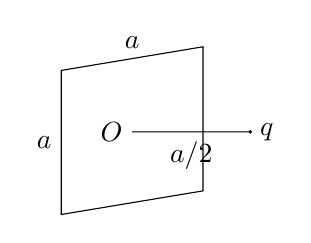
\begin{tikzpicture}[x=15mm,y=15mm]
	\draw(-.6,-.7)--++(1.2,.2)--++(0,1.22)--node[above]{$a$}++(-1.2,-.2)--node[left]{$a$}cycle;
	\draw(0,0)node[left]{$O$}--node[below]{$a/2$}+(1,0)[fill=black]circle(.01)node[right]{$q$};
\end{tikzpicture}
\end{document}
